\chapter{Objetivos}
\label{ch:Objetivos}

Una vez presentado el contexto de este TFG, fijamos ahora los objetivos concretos que se han abordado. También se describe la metodología de trabajo seguida y la planificación temporal.

\section{Descripción del problema}
\label{sec:obj_descripcionproblema}

El objetivo principal de este trabajo consiste en mejorar y ampliar la colección de prácticas de JdeRobot-Academy, enriqueciéndolas y aumentando el abanico de posibilidades que se ofrece al alumno. Para ello necesitamos entender el funcionamiento tanto de JdeRobot como de ROS y familiarizarnos con el manejo de programas de edición 3D. Este objetivo lo hemos dividido en dos principales que constituirán nuevas prácticas para el entorno docente:
\begin{itemize}
	\item Mejorar la infraestructura en Gazebo de las prácticas de JdeRobot-Academy que usan coches de carreras: Crearemos un modelo 3D de un escenario real con elevaciones para realizar las prácticas de JdeRobot-Academy en las que se usa un Fórmula 1, aquella en la que ha de seguir una línea y aquella en la que ha de dar vueltas esquivando obstáculos. Elegimos el circuito de Fórmula 1 de Mónaco por ser un circuito conocido, corto tanto en su longitud como en el área que ocupa, y por estar ubicado en un entorno urbano y montañoso, lo que hace que sea estrecho y con subidas y bajadas. Lo prepararemos para estas dos prácticas específicas, añadiendo barreras en los bordes de la pista o marcas en el asfalto, y lo construiremos de forma que sea sencillo realizar futuras modificaciones para otros tipos de prácticas.
	
	\item Diseñar y programar un teleoperador de un brazo robótico en Gazebo: Buscaremos un brazo robótico que funcione en Gazebo y bajo ROS. Analizaremos su construcción y su funcionamiento y construiremos un controlador de bajo nivel que actúe directamente sobre las partes móviles del brazo, es decir, que mueva las articulaciones una a una. Para ello estudiaremos la interfaz de manejo que ofrece el entorno ROS para estos robots articulados. Crearemos una ventana con unos controles intuitivos para facilitar el manejo del robot.
\end{itemize}

\subsection{Requisitos}
\label{subsec:obj_requisitos}
 Además de alcanzar los objetivos marcados, las soluciones alcanzadas deberán cumplir estos requisitos:
\begin{itemize}
	\item El desarrollo de este proyecto funcionará para la versión 5.5 del entorno JdeRobot, así como bajo Gazebo 7 y ROS Kinetic. Los componentes software se programarán utilizando principalmente Python, y en aquellos casos que no sea posible, utilizando el lenguaje principal de la plataforma o del tipo de archivo necesario.
	
	\item El coste computacional de los mundos 3D creados para Gazebo deberá estar acotado, en la medida de lo posible, para que sea usable desde ordenadores normales, habituales entre los alumnos o en los laboratorios. 
	
	\item Los mundos creados se incorporarán al repositorio oficial de JdeRobot, por lo que debe ser posible utilizarlos junto con la plataforma de forma eficiente y estar afinados para su uso por terceros.

\end{itemize}

\section{Metodología}
\label{sec:obj_metodologia}


En el desarrollo del software de los componentes de nuestro trabajo utilizamos un  modelo de ciclo de vida en espiral. Es un modelo de proceso de software evolutivo, desarrollado por primera vez por Barry Boehm en 1988. En este modelo las actividades a realizar se conforman siguiendo una espiral, en la que cada bucle o iteración representa un conjunto de actividades que completan un modelo del proyecto final. Proporciona un modo de desarrollo evolutivo con un coste y complejidad incremental. 

Usando este modelo, al final de cada iteración obtenemos un prototipo funcional que cumple los requisitos marcados para esa iteración, lo que nos permite desarrollar poco a poco los objetivos. De esta manera aseguramos funcionalidades en cada paso y llevamos un seguimiento más preciso de fallos y bugs. También nos permite adaptarnos mejor a cambios de planificación y de requisitos.

\begin{figure}[hb]
	\centering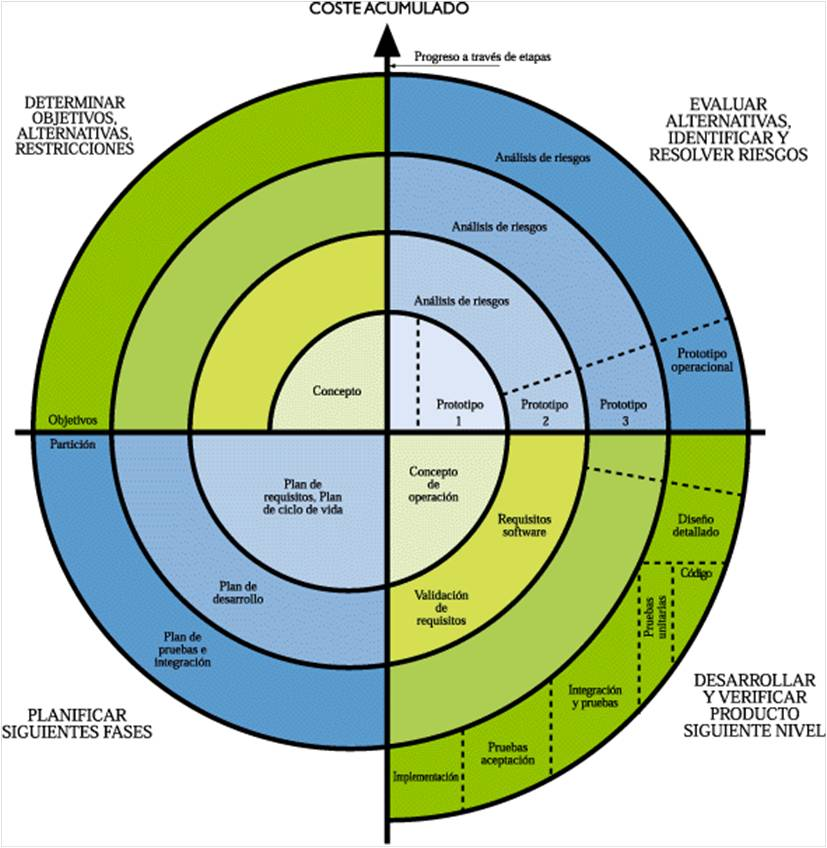
\includegraphics[width=0.7\textwidth]{espiral.jpg}
	\caption{Modelo de ciclo de vida en espiral.}
	\label{fig:espiral}
\end{figure}

En cada vuelta de la espiral se parte de los resultados obtenidos en la anterior y se aumenta la complejidad. Dentro de cada vuelta se siguen una serie de pasos o tareas que guían el desarrollo del proyecto en cada iteración, como muestra el esquema que podemos ver en la figura \ref{fig:espiral}, Los pasos son:
\begin{enumerate}[1.]
	\item Determinar objetivos, alternativas, restricciones: En este paso se definen los objetivos específicos que tendremos que cumplir en cada iteración teniendo en mente el resultado final del proceso. Además se diseña una planificación detallada de gestión y se identifican las posibles alternativas. 
	
	\item Evaluar alternativas, identificar y resolver riesgos: Se efectúa un análisis detallado de las posibles alternativas que nos permitan cumplir los objetivos marcados utilizando distintos puntos de vista. Además se tienen en cuenta los riesgos del proceso, se elige la mejor estrategia teniendo en cuenta las dificultades que puedan surgir y se plantean estrategias alternativas para paliar el impacto de estos problemas.
	
	\item Desarrollar y verificar producto: Se desarrolla el producto de acuerdo a la planificación efectuada apuntando a los objetivos propuestos dentro del ciclo. Seguidamente probamos que el resultado sea satisfactorio de acuerdo a dichos objetivos.
	
	\item Planear las siguientes fases: Se revisa el proyecto y se decide si continuar con un nuevo ciclo de la espiral. En caso afirmativo se desarrollan los planes para la siguiente iteración y se subsanan los posibles errores cometidos en la última iteración.
	
\end{enumerate}

Se han realizado reuniones semanales con el tutor para mantener un seguimiento y una progresión adecuada en el desarrollo del proyecto, alcanzando los objetivos marcados y estudiando diferentes alternativas para conseguirlos.

Para tener constancia de los progresos y del desarrollo general del proyecto se ha utilizado un apartado en la propia página de JdeRobot, un MediaWiki\cite{mediawiki} donde ir documentando periódicamente los progresos, incluyendo fotos y vídeos de los logros conseguidos y de los problemas encontrados. Ha servido como referencia para que las reuniones con el tutor estén sincronizadas, y a modo de diario para mantener un registro de los progresos y de las dificultades encontradas. También se ha utilizado un repositorio en GitHub\cite{mirepo} donde se encuentran todos los archivos relacionados con el proyecto, desde test y tutoriales hasta el código fuente del resultado final, pasando por alternativas descartadas y pruebas fallidas.

\section{Planificación temporal}
\label{sec:obj_planificaciontemporal}

Las fases de desarrollo seguidas en el proyecto se corresponden con los pasos seguidos en los siguientes capítulos. Las principales son:

\begin{itemize}
	\item Estudio del entorno JdeRobot:
	En esta primera fase nos centraremos en entender el funcionamiento del entorno JdeRobot y de integrarnos en el grupo de robótica. Estudiaremos los diversos componentes que forman el entorno y qué papel desempeña cada uno, centrándonos en los mundos de Gazebo y los plugins de control de los robots ya que son los elementos que más en profundidad desarrollaremos en nuestro proyecto. Para ello recurrimos a los múltiples ejemplos facilitados y a la lista de correo del grupo de robótica, la cuál resultó ser de una ayuda inestimable para solucionar los problemas surgidos en estos primeros compases del proyecto.
	
	\item Desarrollo del circuito realista de Fórmula 1:
	En esta segunda fase nos familiarizamos con el manejo de Blender, una herramienta potente pero muy diferente a los editores habituales de texto o de imágenes. Recurrimos a diversos tutoriales encontrados en su página centrándonos en el modelado de objetos 3D, ya que características como la animación, la simulación de fluidos o el desarrollo de videojuegos no son necesarias en este proyecto. Nos familiarizamos con el tratamiento de imagen para las texturas, buscando formas de conseguirlas y de editarlas para aplicarlas al circuito. También fue necesaria una investigación sobre las características topológicas del circuito para darle mayor realismo, tanto en la configuración del trazado como en las elevaciones del terreno.
	
	\item Estudio de ROS y ARIAC:
	Al igual que con el entorno de JdeRobot, necesitamos estudiar el funcionamiento de ROS para comprenderlo y aplicarlo en la realización del teleoperador. Encontramos en su extensa documentación y tutoriales toda la información que necesitamos. También estudiamos los componentes que forman ARIAC para comprender su funcionamiento y cómo usar ROS para manejar el brazo. A través de sus tutoriales vemos que ofrece la posibilidad de utilizar planificadores de movimiento como MoveIt, que forman parte de los complementos de ROS, por lo que indagamos más en ellos.
	
	\item Desarrollo del teleoperador:
	Cuando ya hemos adquirido los conocimientos sobre ROS y ARIAC necesarios comenzamos el desarrollo del teleoperador. Para ello repasamos el lenguaje Python y comenzamos dando pequeños pasos para afianzar los conocimientos sobre ROS y relacionarlos con el mundo de ARIAC y el brazo que contiene. Al finalizar realizamos pruebas para comprobar que el funcionamiento es el adecuado y se comporta como esperábamos.
	
	\item Documentación del proyecto:
	Para finalizar, una vez alcanzados los objetivos planteados comenzamos con la escritura de la memoria. Nos apoyamos en el MediaWiki que hemos escrito a medida que realizábamos progresos en el trabajo para recordar los pasos seguidos y las fuentes consultadas.
	
\end{itemize}




